\section{Scene Distance Measure}
Borrowing the methodology from Pop-Share, we compare videos without revealing their content, specifically examining both identical and different scenes. Using the supervised labeling from the experiments in Section 5.3, where a label of one indicates the same scene and zero indicates different scenes, Figure \ref{fig:scene-distance-measure} illustrates the average Distance Measure for all three algorithms. 

\begin{figure}[ht]
    \centering
    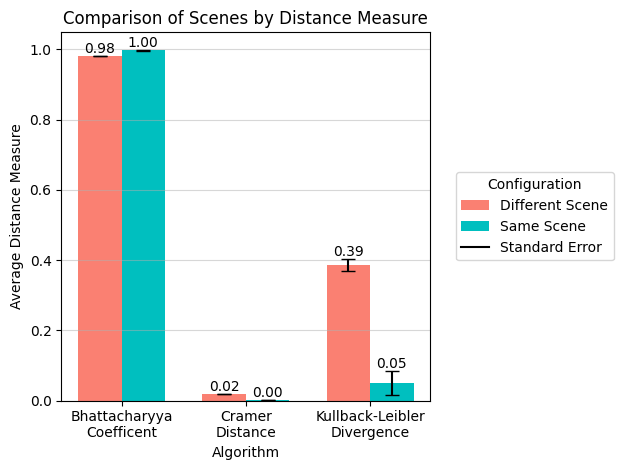
\includegraphics[width=0.8\textwidth]{5 Results/Figures/5.4 Bar Chart.png}
    \caption{Scene Distance Measure}
    \label{fig:scene-distance-measure}
\end{figure}

For the Bhattacharyya Coefficient, a perfect score of 1.00 indicates that the two scenes are identical, while a score of zero denotes no overlap. For Cramer Distance, a perfect score of 0.00 indicates that the two scenes are identical, while a score of 1.0 is the maximum distance between two probability distributions. In our experiments, we observed a 0.02 variance between the distance measures for different and same scenes. This minimal variance is likely attributed to the uniformity of the scene types recorded, as both sets were filmed indoors, and the fact that the same devices were used during the experiments, which limited the diversity in the captured footage.

For the Kullback-Leibler Divergence (KLD), a perfect score of 0.00 indicates that two scenes are identical, while the upper limit is infinity; the smaller the score, the more similar the two probability distributions are. In our experiments, we observed a 0.34 variance between the distance measures for different and same scenes. This represents the highest variance observed among all of our distance measures and serves as a significant indicator that two scenes may be different.
The key takeaway from our experiments is that while the individual scores for the distance measures exhibit minimal variance, they still effectively differentiate between identical and different scenes. This consistency suggests that the implemented algorithms can reliably assess similarity, even in scenarios where the overall variation in scores is low. Consequently, the results highlight the robustness of our methodology in accurately identifying scene differences, which is crucial for applications requiring precise content analysis without revealing the underlying video data.
